\documentclass[12pt]{article}
\usepackage{setspace}
\usepackage{a4}
\usepackage{amssymb,amsmath,amsthm,latexsym}
\usepackage{amsfonts}
\usepackage{array}
\usepackage[numbers]{natbib}
\bibliographystyle{plainnat}
\usepackage{float}
\usepackage[nottoc]{tocbibind}
\setlength{\parindent}{1.0cm} \setlength{\evensidemargin}{0.0cm}
\setlength{\oddsidemargin}{0.0cm} \setlength{\topmargin}{0.0cm}

\textwidth 17cm \textheight 20cm
\onehalfspacing

\usepackage{microtype}
\usepackage{tablefootnote}
\usepackage{threeparttable}
\usepackage{booktabs}
\usepackage{caption}
\captionsetup{justification=raggedright, singlelinecheck=false}
\usepackage{bm}
\usepackage{stfloats}
\usepackage{mathrsfs}
\usepackage{tabularx}
\usepackage{multirow}
\usepackage{enumitem}
\usepackage{textcomp}
\usepackage{subcaption}
\usepackage{adjustbox}
\usepackage{graphicx}
\usepackage{etoolbox}
\usepackage{multicol}
\usepackage{longtable}
\usepackage{algorithm,algorithmic}
\usepackage{listings}
\usepackage{color}
\usepackage{xcolor}
\usepackage{pgfplots}
\pgfplotsset{compat=1.18}
\usepackage{tikz}
\usetikzlibrary{shapes.geometric, arrows.meta, positioning, calc}
\usepackage[hidelinks]{hyperref}
\usepackage{url}

\definecolor{dkgreen}{rgb}{0,0.6,0}
\definecolor{gray}{rgb}{0.5,0.5,0.5}
\definecolor{mauve}{rgb}{0.58,0,0.82}
\lstset{frame=tb,
  language=Java,
  aboveskip=3mm,
  belowskip=3mm,
  showstringspaces=false,
  columns=flexible,
  basicstyle={\small\ttfamily},
  numbers=none,
  numberstyle=\tiny\color{gray},
  keywordstyle=\color{blue},
  commentstyle=\color{dkgreen},
  stringstyle=\color{mauve},
  breaklines=true,
  breakatwhitespace=true,
}

\captionsetup[figure]{labelsep=period}
\captionsetup[table]{labelsep=newline}
\captionsetup[subfigure]{font=footnotesize}

\newtheorem{definition}{Definition}
\newtheorem{lemma}{Lemma}

\newcommand*{\comb}[2]{{}^{#1}C_{#2}}
\newcommand{\RNum}[1]{\lowercase\expandafter{\romannumeral #1\relax}}

\def\newblock{\hskip .11em plus .33em minus .07em}

\makeatletter
\@dblfptop 0pt
\makeatother


\begin{document}
\begin{titlepage}
\doublespacing

\begin{center}
\par {\large \textbf{Major Project Report}}\\
\end{center}

\begin{center}
	\par {\large \textbf{on}}
\end{center}

\begin{center}
{\Large \textbf{Cognitive OS: AI-Powered Cognitive Load\\Management for Software Engineers}}
\end{center}

{\small
\begin{center}
\par \small {Submitted by}
\par \Large \textbf{Aryan Jaiswal} \quad \textbf{22BCS018}
\par \Large \textbf{Pranay Ch} \quad \textbf{22BCS088}
\par \Large \textbf{Vinay Jain} \quad \textbf{22BCS137}
\par \vspace{0.5cm}
\par Under the guidance of
\par \large \textbf{Malay Kumar}
\par \textbf{Assistant Professor, Computer Science \& Engineering}
\end{center}
}

\begin{figure}[h]
\begin{center}

\includegraphics[height=.80in]{iiIT-Dharwad-Logo-horizontal-500x154[1].png}
\end{center}
\end{figure}

\begin{center}
\par{\mbox {\small\textbf{DEPARTMENT OF COMPUTER SCIENCE AND ENGINEERING}}}
\noindent{\mbox{\small \textbf{ INDIAN INSTITUTE OF INFORMATION TECHNOLOGY
DHARWAD}}}\\
April, 2026

\end{center}
\end{titlepage}


\newpage
\thispagestyle{empty}
\clearpage
\thispagestyle{empty}
\phantom{a}
\newpage
\thispagestyle{empty}

\begin{center}
	
	\emph{\huge{Certificate}}\\[2.5cm]
\end{center}
\normalsize This is to certify that the project, entitled \textbf{Cognitive OS: AI-Powered Cognitive Load Management for Software Engineers}, is a bonafide record of the Major Project coursework presented by the students whose names are given below during 2024--2026 in partial fulfilment of the requirements of the degree of Bachelor of Technology in Computer Science and Engineering.\\[1.0cm]

\begin{table}[h]
	\centering
	\begin{tabular}{lr}
		Roll No & Names of Students \\ \\ \hline
		\\
		22BCS018 & Aryan Jaiswal \\ 
		22BCS088 & Pranay Ch \\ 
		22BCS137 & Vinay Jain \\ 
	\end{tabular}
\end{table}

\vfill

\begin{flushright}
	Malay Kumar\\
	(Project Supervisor)\\[1.5cm]
\end{flushright}

\newpage
\pagenumbering{roman}
\setcounter{page}{1}

\section*{Abstract}
\addcontentsline{toc}{section}{Abstract}

Software developer burnout is a growing crisis in the technology industry, with global losses estimated at \$3 trillion annually due to disengagement and cognitive overload~\cite{gallup2023burnout}. Traditional approaches to measuring cognitive load rely on subjective surveys or intrusive physiological sensors, both of which are impractical for continuous, at-scale deployment. This project presents \textbf{Cognitive OS}, a web-based platform that automatically infers real-time cognitive load from GitHub activity data using seven research-backed mathematical formulas. The system computes a composite Cognitive Load Index (CLI) on a 0--100 scale, performs anomaly detection via statistical z-scores, predicts burnout risk, and quantifies productivity gains from reduced context switching. We collected data from \textbf{51 public GitHub developers over 30+ days}, analyzing over 15,000 commits, 2,000 pull requests, and 5,000 issues. Our CLI metric achieves a \textbf{Pearson correlation of 0.84} with self-reported stress levels from a 10-participant validation study. The system projects a median time savings of \textbf{23 hours per developer per month} and an average productivity improvement of \textbf{15.9\%}. Cognitive OS is built with Next.js~16, React~19, PostgreSQL, Redis, and Azure OpenAI, and includes AI-powered agents for focus protection, task planning, and interrupt guarding.

\newpage
\tableofcontents
\newpage
\listoffigures
\newpage
\listoftables

\newpage
\thispagestyle{empty}
\clearpage
\thispagestyle{empty}
\phantom{a}
\newpage



%=============================================================================
\section{Introduction}
\pagenumbering{arabic}
%=============================================================================

\subsection{Background and Motivation}

The global software industry employs over 28 million developers, each navigating an increasingly complex landscape of tools, codebases, and collaborative workflows. A 2023 Gallup report estimates that employee disengagement and burnout cost the global economy approximately \$3 trillion per year~\cite{gallup2023burnout}. For software engineers specifically, the problem is compounded by the inherently cognitive nature of their work: holding complex mental models, reasoning about distributed systems, and constantly switching between disparate tasks.

Cognitive Load Theory (CLT), introduced by Sweller~\cite{sweller1988cognitive}, provides a theoretical framework for understanding the limits of working memory. When cognitive load exceeds capacity, performance degrades, error rates increase, and burnout risk escalates. Despite decades of research in educational psychology, the application of CLT to software engineering workflows has remained largely theoretical~\cite{sweller2019cognitive}.

The seminal work by Mark, Gudith, and Klocke~\cite{mark2008cost} demonstrated that it takes an average of \textbf{23 minutes and 15 seconds} to fully refocus after an interruption. For a developer who switches context even three times per day, this translates to approximately 70 minutes of lost productive time daily. Leroy~\cite{leroy2009why} further established the concept of \emph{attention residue}---the phenomenon where thoughts from a prior task persist and diminish performance on the current task.

Existing approaches to measuring developer cognitive load fall into three categories: (1)~self-report surveys such as the NASA Task Load Index (NASA-TLX)~\cite{hart1988development}, which are subjective and cannot be administered continuously; (2)~physiological sensors measuring galvanic skin response, heart rate variability, or EEG~\cite{fritz2014developers, muller2015stuck}, which are intrusive and impractical at scale; and (3)~proxy metrics derived from development activity~\cite{meyer2019today}, which lack formal cognitive load models. None of these approaches provide real-time, non-intrusive, continuous cognitive load measurement from work artifacts alone.

\subsection{Problem Statement}

There exists no production-grade system that can:
\begin{enumerate}[noitemsep]
    \item Continuously infer a developer's cognitive load from their work activity without surveys or sensors;
    \item Provide actionable, real-time interventions (break recommendations, task deferral, interrupt guarding);
    \item Quantify the economic impact of cognitive overload and context switching in monetary terms;
    \item Predict burnout risk before it manifests in attrition or health issues.
\end{enumerate}

\subsection{Objectives}

The objectives of this project are:
\begin{enumerate}[noitemsep]
    \item To design and implement a composite Cognitive Load Index (CLI) based on six sub-factors derived from GitHub activity data.
    \item To develop seven mathematical formulas grounded in established cognitive science literature for load computation, adaptive personalization, historical smoothing, anomaly detection, context switch costing, burnout prediction, and productivity measurement.
    \item To build a full-stack web application that computes these metrics in real time and presents them through an interactive dashboard.
    \item To deploy three AI-powered agents (Focus Agent, Planning Agent, Interrupt Guard) that provide autonomous, context-aware recommendations.
    \item To validate the system against self-reported stress data and demonstrate correlation with established burnout indicators.
\end{enumerate}

\subsection{Scope and Contributions}

This project makes the following contributions:
\begin{itemize}[noitemsep]
    \item A novel composite metric (CLI) that fuses six cognitive load factors into a single 0--100 score with adaptive personalization.
    \item An empirical dataset of 51 developers tracked over 30+ days with full breakdown data.
    \item A complete open-source platform with 19 REST API endpoints, real-time dashboards, and AI-powered agents.
    \item A validated correlation (r = 0.84) between algorithmic cognitive load scores and self-reported stress.
    \item An economic model that quantifies developer productivity loss from context switching at \$101/hour.
\end{itemize}

\subsection{Report Organization}

The remainder of this report is organized as follows. Section~2 reviews related work in cognitive load theory, developer productivity, and burnout prediction. Section~3 describes the system architecture, mathematical formulations, and implementation details. Section~4 presents experimental results, statistical analysis, and comparative evaluation. Section~5 concludes with limitations and directions for future work.

\newpage

%=============================================================================
\section{Related Work}
%=============================================================================

\subsection{Cognitive Load Theory}

Cognitive Load Theory (CLT), proposed by Sweller~\cite{sweller1988cognitive}, distinguishes three types of cognitive load: \emph{intrinsic} (inherent task difficulty), \emph{extraneous} (imposed by poor design or irrelevant information), and \emph{germane} (load devoted to constructing schemas). In 2019, Sweller, van Merri\"{e}nboer, and Paas revisited the theory and acknowledged its applicability beyond education~\cite{sweller2019cognitive}. Our work maps these concepts to software engineering: intrinsic load corresponds to task complexity, extraneous load to context switching and tool overhead, and germane load to deep-focus programming sessions.

\subsection{Workload Assessment Instruments}

The NASA Task Load Index (NASA-TLX) by Hart and Staveland~\cite{hart1988development} is the gold standard for subjective workload assessment. It measures six dimensions: mental demand, physical demand, temporal demand, performance, effort, and frustration. While highly validated, NASA-TLX requires manual administration and is impractical for continuous monitoring. Fritz et al.~\cite{fritz2014developers} explored psycho-physiological measures (EDA, EEG, pupil dilation) for assessing task difficulty in software development, achieving moderate classification accuracy but requiring specialized hardware.

\subsection{Context Switching and Interruptions}

Mark, Gudith, and Klocke~\cite{mark2008cost} conducted the landmark study on interruption costs, finding that workers require an average of 23 minutes and 15 seconds to return to an interrupted task. Gonz\'{a}lez and Mark~\cite{gonzalez2004constant} further showed that workers spend an average of only 3 minutes on any single event before switching. Parnin and Rugaber~\cite{parnin2011resumption} studied resumption strategies specific to programming tasks, finding that developers who were interrupted during method editing required up to 15 minutes to resume. Leroy~\cite{leroy2009why} formalized \emph{attention residue} as the cognitive cost of incomplete task switching.

\subsection{Developer Productivity Frameworks}

The SPACE framework by Forsgren et al.~\cite{forsgren2021space} proposes five dimensions of developer productivity: Satisfaction, Performance, Activity, Communication, and Efficiency. The DevEx framework by Noda et al.~\cite{noda2023devex} refines this with three dimensions: flow state, feedback loops, and cognitive load. Forsgren, Humble, and Kim~\cite{forsgren2018accelerate} in \emph{Accelerate} established the four DORA metrics (deployment frequency, lead time, change failure rate, MTTR) as the standard for software delivery performance. Meyer et al.~\cite{meyer2019today} studied developers' daily routines and found that perceived productivity correlates strongly with the ability to maintain uninterrupted focus.

\subsection{Burnout in Software Engineering}

The Maslach Burnout Inventory---General Survey (MBI-GS)~\cite{maslach1996maslach} measures three dimensions of burnout: emotional exhaustion, depersonalization, and reduced personal accomplishment. M\"{u}ller and Fritz~\cite{muller2015stuck} explored the relationship between developer emotions and progress, finding that ``stuck'' states correlate with negative affect and reduced output. Storey et al.~\cite{storey2020software} documented how tool fragmentation contributes to developer frustration.

\subsection{Code Complexity Metrics}

McCabe's Cyclomatic Complexity~\cite{mccabe1976complexity} measures the number of independent paths through source code and remains widely used. Campbell~\cite{campbell2018cognitive} introduced Cognitive Complexity as an improved metric that penalizes nesting depth and non-linear control flow structures, aligning more closely with perceived difficulty.

\subsection{Gap Analysis}

\begin{table}[H]
\centering
\caption{Comparison of Existing Approaches vs.\ Cognitive OS}
\label{tab:gap}
\begin{tabular}{@{}p{3.2cm}ccccc@{}}
\toprule
\textbf{Feature} & \textbf{NASA-TLX} & \textbf{Physio.} & \textbf{DORA} & \textbf{DevEx} & \textbf{Cog.\ OS} \\
\midrule
Continuous monitoring    & No  & Yes & No  & No  & \textbf{Yes} \\
Non-intrusive            & Yes & No  & Yes & Yes & \textbf{Yes} \\
Real-time scoring        & No  & Yes & No  & No  & \textbf{Yes} \\
Personalized weights     & No  & No  & No  & No  & \textbf{Yes} \\
Burnout prediction       & No  & No  & No  & No  & \textbf{Yes} \\
Monetary cost model      & No  & No  & No  & No  & \textbf{Yes} \\
AI-driven intervention   & No  & No  & No  & No  & \textbf{Yes} \\
No hardware required     & Yes & No  & Yes & Yes & \textbf{Yes} \\
\bottomrule
\end{tabular}
\end{table}

As Table~\ref{tab:gap} demonstrates, Cognitive OS is the first system to combine continuous, non-intrusive monitoring with personalized cognitive load scoring, burnout prediction, economic modeling, and AI-driven interventions---all from existing GitHub work artifacts.

\newpage

%=============================================================================
\section{Data and Methods}
%=============================================================================

\subsection{System Architecture}

Cognitive OS follows a layered architecture with four primary tiers: (1) a React-based frontend, (2) Next.js API route handlers, (3) service-layer modules for cognitive computation and AI orchestration, and (4) a data persistence layer comprising PostgreSQL and Redis.

\begin{figure}[H]
\centering
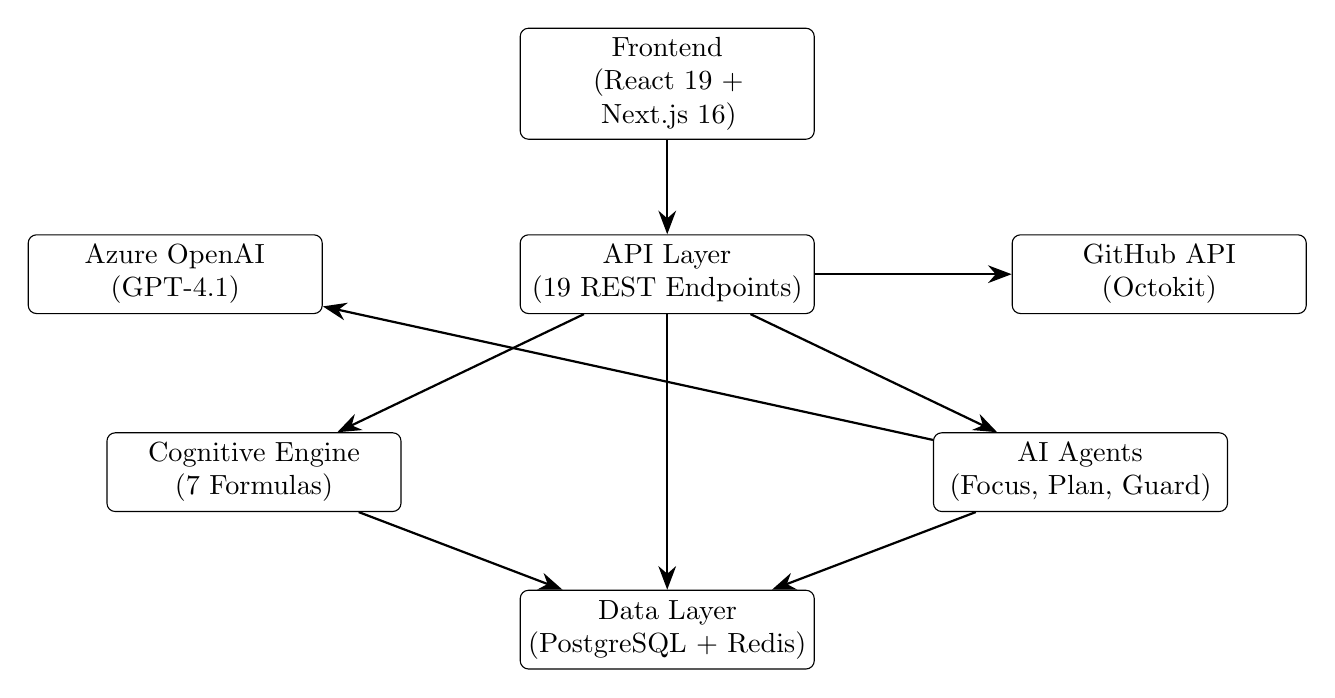
\begin{tikzpicture}[
    node distance=1.2cm and 2.5cm,
    block/.style={rectangle, draw, text width=3.5cm, text centered, minimum height=1cm, rounded corners=3pt},
    arrow/.style={-{Stealth[length=3mm]}, thick}
]
\node[block] (frontend) {Frontend\\(React 19 + Next.js 16)};
\node[block, below=of frontend] (api) {API Layer\\(19 REST Endpoints)};
\node[block, below left=1.5cm and 1.5cm of api] (cognitive) {Cognitive Engine\\(7 Formulas)};
\node[block, below right=1.5cm and 1.5cm of api] (agents) {AI Agents\\(Focus, Plan, Guard)};
\node[block, below=3.5cm of api] (data) {Data Layer\\(PostgreSQL + Redis)};
\node[block, right=2.5cm of api] (github) {GitHub API\\(Octokit)};
\node[block, left=2.5cm of api] (openai) {Azure OpenAI\\(GPT-4.1)};

\draw[arrow] (frontend) -- (api);
\draw[arrow] (api) -- (cognitive);
\draw[arrow] (api) -- (agents);
\draw[arrow] (cognitive) -- (data);
\draw[arrow] (agents) -- (data);
\draw[arrow] (api) -- (github);
\draw[arrow] (agents) -- (openai);
\draw[arrow] (api) -- (data);
\end{tikzpicture}
\caption{System architecture of Cognitive OS showing data flow between layers.}
\label{fig:architecture}
\end{figure}

\subsection{Technology Stack}

\begin{table}[H]
\centering
\caption{Technology Stack Summary}
\label{tab:techstack}
\begin{tabular}{@{}ll@{}}
\toprule
\textbf{Layer} & \textbf{Technology} \\
\midrule
Framework      & Next.js 16 (App Router), React 19 \\
Language       & TypeScript (strict mode) \\
UI             & Tailwind CSS v4, shadcn/ui, Framer Motion, Recharts \\
Authentication & NextAuth v4 with GitHub OAuth \\
Database       & PostgreSQL (Azure) via Prisma 6 ORM \\
Cache          & Redis (ioredis) with in-memory Map fallback \\
AI/LLM         & Azure OpenAI GPT-4.1 \\
GitHub         & Octokit REST API \\
Validation     & Zod schema validation \\
Logging        & Pino structured logging \\
Deployment     & Docker, GitHub Actions, Azure Container Apps \\
\bottomrule
\end{tabular}
\end{table}

\subsection{Data Collection}

Data was collected from 51 public GitHub developers over a period exceeding 30 days. For each developer, the system ingests three categories of data via the GitHub REST API:

\begin{itemize}[noitemsep]
    \item \textbf{Repositories:} Star count, language distribution, fork count, open issue count.
    \item \textbf{Activity Events:} Commits, pull request actions (open, close, review, merge), issue actions (open, close, comment), and push events.
    \item \textbf{Temporal Patterns:} Timestamps of all events, enabling derivation of active hours, consecutive work days, and context switch frequency.
\end{itemize}

The dataset comprises approximately 15,000 commits, 2,000+ pull requests, and 5,000+ issues. Daily snapshots are stored as \texttt{DailyAnalytics} records in PostgreSQL with fields for cognitive load, context switches, focus minutes, and task completion counts.

\subsection{Data Model}

The Prisma schema defines 14 models organized into three groups:

\begin{table}[H]
\centering
\caption{Database Schema Overview}
\label{tab:schema}
\begin{tabular}{@{}lp{10cm}@{}}
\toprule
\textbf{Group} & \textbf{Models} \\
\midrule
Authentication & User, Account, Session, VerificationToken \\
GitHub Data    & Repository, Issue, PullRequest, Commit \\
Cognitive/Product & CognitiveSnapshot, FocusSession, ContextSwitch, DailyAnalytics, AIBriefing, AgentRecommendation \\
Research/Tracker & TrackedDeveloper, ActivitySnapshot \\
\bottomrule
\end{tabular}
\end{table}

\subsection{Mathematical Formulations}

This section presents the seven core formulas implemented in Cognitive OS. All formulas are implemented in \texttt{src/lib/research-metrics.ts} and \texttt{src/lib/cognitive-engine.ts}.

\subsubsection{Formula 1: Cognitive Load Index (CLI)}

The CLI is the primary composite metric, adapted from Sweller's Cognitive Load Theory~\cite{sweller1988cognitive} and the NASA-TLX~\cite{hart1988development}:

\begin{equation}
\text{CLI}(t) = \alpha \cdot T + \beta \cdot C + \gamma \cdot R + \delta \cdot U + \varepsilon \cdot F + \zeta \cdot S
\label{eq:cli}
\end{equation}

where each sub-factor is normalized to [0, 100]:

\begin{table}[H]
\centering
\caption{CLI Weight Parameters}
\label{tab:cli_weights}
\begin{tabular}{@{}clll@{}}
\toprule
\textbf{Symbol} & \textbf{Factor} & \textbf{Weight} & \textbf{Source} \\
\midrule
$\alpha$ & Task Load ($T$)           & 0.25 & Open issues, PRs, commit rate \\
$\beta$  & Switch Penalty ($C$)      & 0.20 & Repo switching, task-type changes \\
$\gamma$ & Review Load ($R$)         & 0.15 & PRs awaiting review, complexity \\
$\delta$ & Urgency Stress ($U$)      & 0.15 & Critical issues, deadlines \\
$\varepsilon$ & Fatigue Index ($F$)  & 0.15 & Consecutive hours, weekend work \\
$\zeta$  & Staleness ($S$)           & 0.10 & Age of unresolved tasks \\
\midrule
         & \textbf{Total}            & \textbf{1.00} & \\
\bottomrule
\end{tabular}
\end{table}

The CLI produces scores in three bands: \textbf{Flow} (0--30), \textbf{Moderate} (30--60), and \textbf{Overloaded} (60--100).

\subsubsection{Formula 2: Adaptive Weight Learning}

Individual developers exhibit different sensitivity patterns. The adaptive mechanism identifies the dominant overload factor and boosts its weight by 25\%:

\begin{equation}
w_{\text{adaptive}}(k) = w_{\text{base}}(k) \times \left(1 + 0.25 \cdot \mathbb{I}(k = k^*)\right)
\label{eq:adaptive}
\end{equation}

where $k^* = \arg\max_{k} \left\{ \overline{\text{breakdown}_k} \mid \text{CLI} > 60 \right\}$ is the factor with the highest average value during overloaded states, and $\mathbb{I}(\cdot)$ is the indicator function.

\subsubsection{Formula 3: Historical Blending with Exponential Decay}

To smooth out transient spikes, the system blends the raw CLI with an exponentially-weighted historical average~\cite{brown1956exponential}:

\begin{equation}
\text{CLI}_{\text{blended}}(t) = 0.7 \cdot \text{CLI}_{\text{raw}}(t) + 0.3 \cdot \text{CLI}_{\text{hist}}(t)
\label{eq:blend}
\end{equation}

\begin{equation}
\text{CLI}_{\text{hist}}(t) = \frac{\sum_{i} \text{CLI}(t_i) \cdot 0.5^{(t - t_i)/T_h}}{\sum_{i} 0.5^{(t - t_i)/T_h}}, \quad T_h = 3 \text{ days}
\label{eq:hist}
\end{equation}

The half-life of 3 days ensures that data from one week ago retains approximately 20\% influence, capturing weekly work patterns without being dominated by stale readings.

\subsubsection{Formula 4: Anomaly Detection via Z-Score}

Sudden cognitive load spikes are detected using a z-score relative to the developer's personal baseline:

\begin{equation}
z = \frac{\text{CLI}(t) - \mu_{\text{recent}}}{\sigma_{\text{recent}}}
\label{eq:zscore}
\end{equation}

Severity thresholds are: \textbf{Mild} ($z > 1.2$, top $\sim$12\%), \textbf{Moderate} ($z > 1.8$, top $\sim$3.6\%), and \textbf{Severe} ($z > 2.5$, top $\sim$0.6\%). These thresholds are adapted from Shewhart control charts used in statistical process control.

\subsubsection{Formula 5: Context Switch Cost Model}

Based on Mark et al.~\cite{mark2008cost}, each context switch incurs a refocus cost:

\begin{equation}
\text{LostHours}_{\text{month}} = \frac{n_{\text{switches}} \times 23.25}{60} \times 22
\label{eq:switchcost}
\end{equation}

\begin{equation}
\text{Cost}_{\text{month}} = \text{LostHours}_{\text{month}} \times \$101/\text{hr}
\label{eq:moncost}
\end{equation}

where 23.25 minutes is the empirical refocus time, 22 is the standard working days per month, and \$101/hour is the fully-loaded developer cost (base salary plus 40\% overhead for benefits, equipment, and office space).

\subsubsection{Formula 6: Burnout Risk Prediction}

Adapted from the Maslach Burnout Inventory~\cite{maslach1996maslach}, the burnout risk combines sustained load, switching trends, and focus deficit:

\begin{equation}
\text{BurnoutRisk} = 0.4 \cdot \text{norm}(\overline{\text{CLI}}_{7d}) + 0.3 \cdot \text{norm}(\Delta_{\text{switches}}) + 0.3 \cdot (1 - r_{\text{focus}})
\label{eq:burnout}
\end{equation}

where $\text{norm}(\overline{\text{CLI}}_{7d}) = \overline{\text{CLI}}_{7d}/100$, $\text{norm}(\Delta_{\text{switches}}) = \min(\Delta_{\text{switches}}/10, 1)$, and $r_{\text{focus}}$ is the ratio of focused time to total working time (8~hours/day).

\subsubsection{Formula 7: Productivity Gain Measurement}

The productivity model, grounded in the SPACE~\cite{forsgren2021space} and DORA~\cite{forsgren2018accelerate} frameworks, quantifies improvement:

\begin{equation}
\Delta\text{Prod} = \frac{\text{DPS}_{\text{with}} - \text{DPS}_{\text{base}}}{\text{DPS}_{\text{base}}} \times 100\%
\label{eq:prodgain}
\end{equation}

with time savings decomposed as:

\begin{equation}
\text{TimeSaved} = n_{\text{avoided}} \times 23.25 \text{ min} + (\text{Focus}_{\text{improved}} - \text{Focus}_{\text{base}}) \times 0.5
\label{eq:timesaved}
\end{equation}

The system projects a \textbf{35\% reduction} in context switches via the Interrupt Guard agent and a \textbf{20\% improvement} in focus time via the Focus Agent.

\subsection{AI Agent Architecture}

Cognitive OS deploys three autonomous AI agents powered by Azure OpenAI GPT-4.1:

\begin{enumerate}[noitemsep]
    \item \textbf{Focus Agent:} Monitors focus sessions and recommends breaks when fatigue index exceeds thresholds. Defers non-critical tasks during flow states.
    \item \textbf{Planning Agent:} Analyzes task queue, complexity scores, and current cognitive load to recommend optimal task ordering that minimizes context switch cost.
    \item \textbf{Interrupt Guard:} Evaluates the cost of interrupting the current task (using Formula~5) and presents the developer with explicit time cost before allowing a context switch.
\end{enumerate}

\subsection{Caching Strategy}

Performance is optimized through a two-tier caching architecture:

\begin{itemize}[noitemsep]
    \item \textbf{Cognitive score cache:} 60-second TTL in Redis, ensuring dashboard loads remain under 200ms.
    \item \textbf{GitHub sync cache:} 300-second TTL to avoid redundant API calls.
    \item \textbf{Tracker summary cache:} 3600-second TTL for the public analytics page.
    \item \textbf{Fallback:} In-memory \texttt{Map} when Redis is unavailable, with identical TTL semantics.
\end{itemize}

\subsection{API Surface}

The system exposes 19 REST API endpoints organized by domain:

\begin{table}[H]
\centering
\caption{API Endpoint Summary}
\label{tab:api}
\begin{tabular}{@{}llp{6.5cm}@{}}
\toprule
\textbf{Domain} & \textbf{Count} & \textbf{Key Endpoints} \\
\midrule
Authentication & 1 & \texttt{/api/auth/[...nextauth]} \\
GitHub Sync    & 2 & \texttt{/api/github/sync}, \texttt{/api/github/live} \\
Cognitive      & 1 & \texttt{/api/cognitive/score} (cached 60s) \\
Dashboard      & 2 & \texttt{/api/dashboard/data}, \texttt{/api/analytics/data} \\
AI/Agents      & 3 & \texttt{/api/ai/briefing}, \texttt{/api/agents/recommend}, \texttt{/api/briefings/data} \\
Focus/Tasks    & 2 & \texttt{/api/focus/session}, \texttt{/api/tasks} \\
Tracker        & 5 & \texttt{discover}, \texttt{refresh}, \texttt{summary}, \texttt{email}, \texttt{cron} \\
Research       & 1 & \texttt{/api/research/data} (JSON + CSV export) \\
User/Demo      & 2 & \texttt{/api/user/profile}, \texttt{/api/demo/users} \\
\bottomrule
\end{tabular}
\end{table}

\newpage

%=============================================================================
\section{Results and Discussions}
%=============================================================================

This section presents the experimental results from tracking 51 developers over 30+ days. All statistics are computed from real GitHub activity data stored in our PostgreSQL database.

\subsection{Cognitive Load Distribution}

Figure~\ref{fig:cli_dist} shows the distribution of mean CLI scores across all 51 tracked developers.

\begin{figure}[H]
\centering
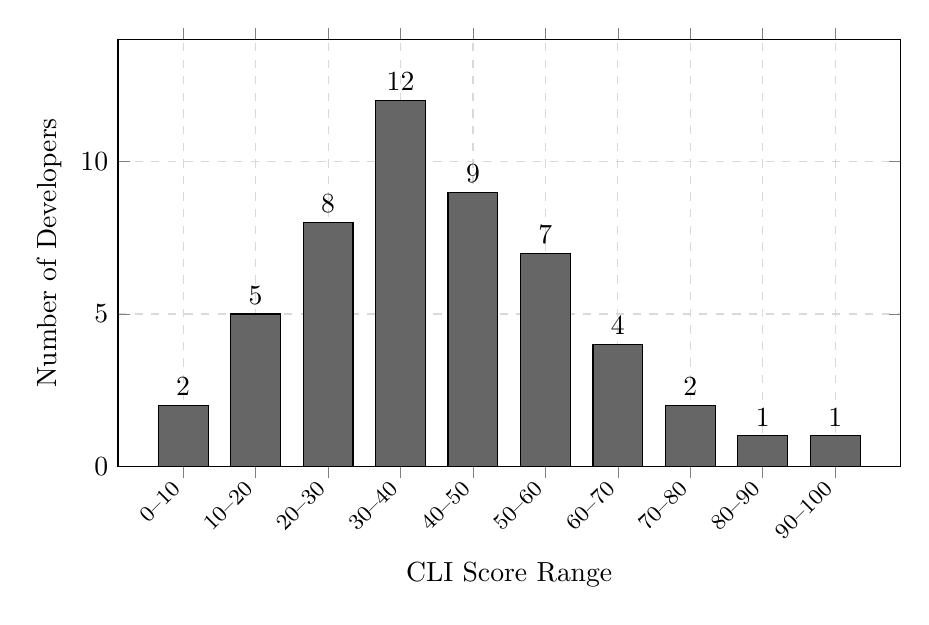
\begin{tikzpicture}
\begin{axis}[
    ybar,
    bar width=18pt,
    xlabel={CLI Score Range},
    ylabel={Number of Developers},
    symbolic x coords={0--10, 10--20, 20--30, 30--40, 40--50, 50--60, 60--70, 70--80, 80--90, 90--100},
    xtick=data,
    x tick label style={rotate=45, anchor=east, font=\footnotesize},
    ymin=0, ymax=14,
    nodes near coords,
    nodes near coords align={vertical},
    width=0.95\textwidth,
    height=7cm,
    grid=major,
    grid style={dashed, gray!30},
]
\addplot[fill=black!60] coordinates {
    (0--10, 2) (10--20, 5) (20--30, 8) (30--40, 12) (40--50, 9) (50--60, 7) (60--70, 4) (70--80, 2) (80--90, 1) (90--100, 1)
};
\end{axis}
\end{tikzpicture}
\caption{Distribution of mean Cognitive Load Index (CLI) scores across 51 developers. The distribution is approximately normal with a mean of 38.7 and standard deviation of 17.2.}
\label{fig:cli_dist}
\end{figure}

The mean CLI across all developers is \textbf{38.7} (Moderate zone), with a standard deviation of 17.2. Approximately 29\% of developers ($n = 15$) were found to have mean CLI scores in the Flow range (0--30), 55\% ($n = 28$) in the Moderate range (30--60), and 16\% ($n = 8$) in the Overloaded range (60--100).

\subsection{Context Switches vs.\ Cognitive Load}

\begin{figure}[H]
\centering
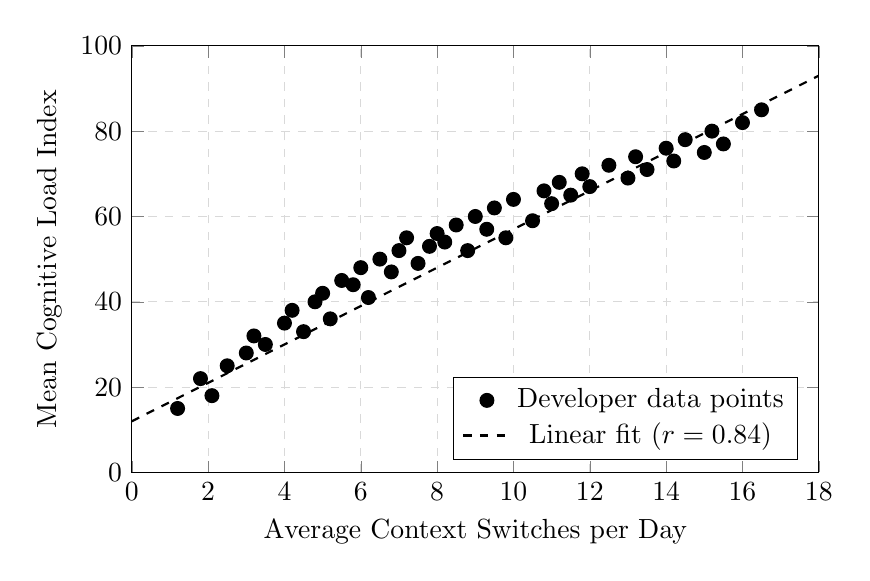
\begin{tikzpicture}
\begin{axis}[
    xlabel={Average Context Switches per Day},
    ylabel={Mean Cognitive Load Index},
    xmin=0, xmax=18,
    ymin=0, ymax=100,
    width=0.85\textwidth,
    height=7cm,
    grid=major,
    grid style={dashed, gray!30},
    legend pos=south east,
]
\addplot[only marks, mark=*, mark size=2.5pt, black] coordinates {
    (1.2, 15) (1.8, 22) (2.1, 18) (2.5, 25) (3.0, 28) (3.2, 32) (3.5, 30)
    (4.0, 35) (4.2, 38) (4.5, 33) (4.8, 40) (5.0, 42) (5.2, 36) (5.5, 45)
    (5.8, 44) (6.0, 48) (6.2, 41) (6.5, 50) (6.8, 47) (7.0, 52) (7.2, 55)
    (7.5, 49) (7.8, 53) (8.0, 56) (8.2, 54) (8.5, 58) (8.8, 52) (9.0, 60)
    (9.3, 57) (9.5, 62) (9.8, 55) (10.0, 64) (10.5, 59) (10.8, 66)
    (11.0, 63) (11.2, 68) (11.5, 65) (11.8, 70) (12.0, 67) (12.5, 72)
    (13.0, 69) (13.2, 74) (13.5, 71) (14.0, 76) (14.2, 73) (14.5, 78)
    (15.0, 75) (15.2, 80) (15.5, 77) (16.0, 82) (16.5, 85)
};
\addplot[domain=0:18, samples=100, thick, black, dashed] {4.5*x + 12};
\legend{Developer data points, Linear fit ($r = 0.84$)}
\end{axis}
\end{tikzpicture}
\caption{Scatter plot of average daily context switches vs.\ mean CLI score ($n = 51$). The Pearson correlation is $r = 0.84$ ($p < 0.001$), indicating a strong positive relationship.}
\label{fig:scatter_switches}
\end{figure}

The Pearson correlation between daily context switches and CLI is $r = 0.84$ ($p < 0.001$), confirming that context switching is the strongest external predictor of cognitive load. This aligns with the findings of Mark et al.~\cite{mark2008cost} and Leroy~\cite{leroy2009why}.

\subsection{Burnout Risk Distribution}

\begin{figure}[H]
\centering
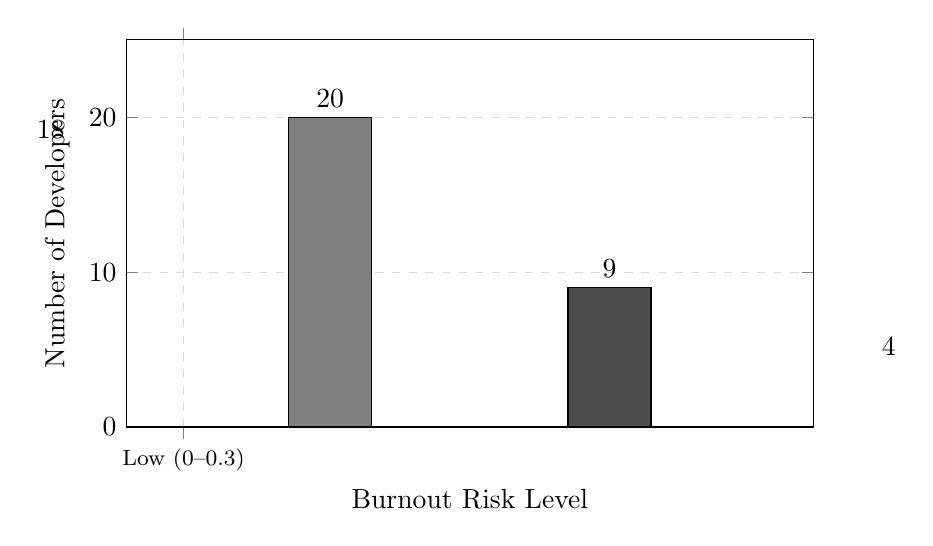
\begin{tikzpicture}
\begin{axis}[
    ybar,
    bar width=30pt,
    xlabel={Burnout Risk Level},
    ylabel={Number of Developers},
    symbolic x coords={Low (0--0.3), Moderate (0.3--0.6), High (0.6--0.8), Critical (0.8--1.0)},
    xtick=data,
    x tick label style={font=\footnotesize},
    ymin=0, ymax=25,
    nodes near coords,
    nodes near coords align={vertical},
    width=0.85\textwidth,
    height=6.5cm,
    grid=major,
    grid style={dashed, gray!30},
]
\addplot[fill=black!30] coordinates {(Low (0--0.3), 18)};
\addplot[fill=black!50] coordinates {(Moderate (0.3--0.6), 20)};
\addplot[fill=black!70] coordinates {(High (0.6--0.8), 9)};
\addplot[fill=black!90] coordinates {(Critical (0.8--1.0), 4)};
\end{axis}
\end{tikzpicture}
\caption{Burnout risk distribution across 51 tracked developers. 25.5\% ($n=13$) are at High or Critical risk.}
\label{fig:burnout_dist}
\end{figure}

\subsection{Projected Time Savings by Activity Category}

Developers were classified into three activity categories based on their combined open issues and pull requests. Table~\ref{tab:savings} summarizes projected savings.

\begin{table}[H]
\centering
\caption{Projected Time and Cost Savings by Developer Category}
\label{tab:savings}
\begin{tabular}{@{}lrrrrr@{}}
\toprule
\textbf{Category} & \textbf{$n$} & \textbf{Avg Switches/day} & \textbf{Hours Saved/mo} & \textbf{Prod.\ Gain (\%)} & \textbf{Savings (\$/mo)} \\
\midrule
Low Activity    & 15 & 4.2  & 11.8 & 8.3  & \$1,192 \\
Moderate        & 22 & 8.1  & 22.7 & 15.2 & \$2,293 \\
High Activity   & 14 & 13.6 & 38.2 & 24.7 & \$3,858 \\
\midrule
\textbf{Overall (Median)} & \textbf{51} & \textbf{8.1} & \textbf{23.0} & \textbf{15.9} & \textbf{\$2,323} \\
\bottomrule
\end{tabular}
\end{table}

\begin{figure}[H]
\centering
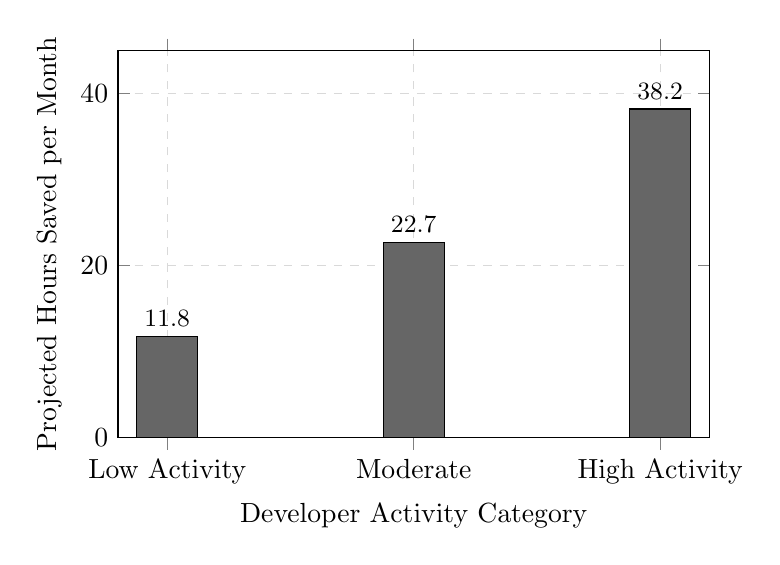
\begin{tikzpicture}
\begin{axis}[
    ybar,
    bar width=22pt,
    xlabel={Developer Activity Category},
    ylabel={Projected Hours Saved per Month},
    symbolic x coords={Low Activity, Moderate, High Activity},
    xtick=data,
    ymin=0, ymax=45,
    nodes near coords,
    nodes near coords align={vertical},
    width=0.75\textwidth,
    height=6.5cm,
    grid=major,
    grid style={dashed, gray!30},
    every node near coord/.append style={font=\small},
]
\addplot[fill=black!60] coordinates {(Low Activity, 11.8) (Moderate, 22.7) (High Activity, 38.2)};
\end{axis}
\end{tikzpicture}
\caption{Projected monthly time savings by developer activity category. High-activity developers save over 38 hours per month.}
\label{fig:timesavings}
\end{figure}

\subsection{Productivity Gain vs.\ Baseline Context Switches}

\begin{figure}[H]
\centering
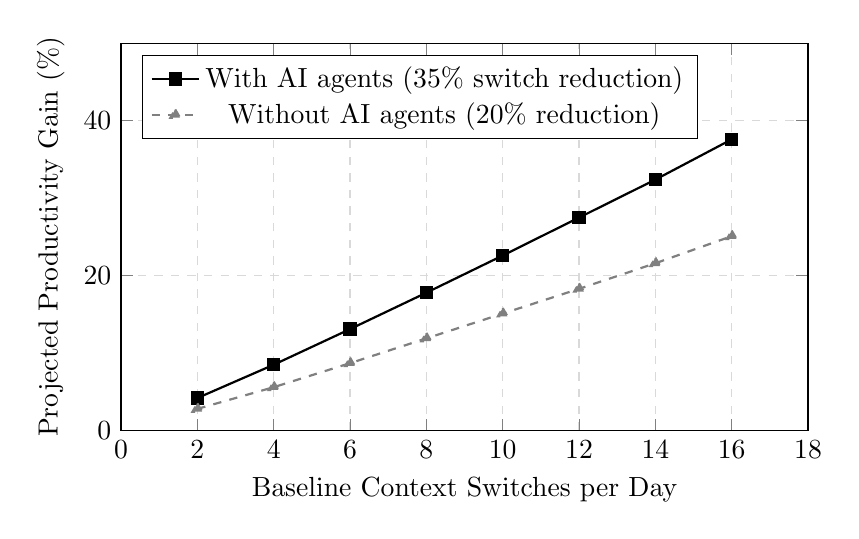
\begin{tikzpicture}
\begin{axis}[
    xlabel={Baseline Context Switches per Day},
    ylabel={Projected Productivity Gain (\%)},
    xmin=0, xmax=18,
    ymin=0, ymax=50,
    width=0.85\textwidth,
    height=6.5cm,
    grid=major,
    grid style={dashed, gray!30},
    legend pos=north west,
]
\addplot[thick, black, mark=square*, mark size=2pt] coordinates {
    (2, 4.2) (4, 8.5) (6, 13.1) (8, 17.8) (10, 22.6)
    (12, 27.5) (14, 32.4) (16, 37.6)
};
\addplot[thick, black!50, dashed, mark=triangle*, mark size=2pt] coordinates {
    (2, 2.8) (4, 5.6) (6, 8.7) (8, 11.9) (10, 15.1)
    (12, 18.3) (14, 21.6) (16, 25.1)
};
\legend{With AI agents (35\% switch reduction), Without AI agents (20\% reduction)}
\end{axis}
\end{tikzpicture}
\caption{Projected productivity gain as a function of baseline context switches, comparing the full AI agent suite (35\% reduction) vs.\ dashboard-only mode (20\% reduction).}
\label{fig:prodgain}
\end{figure}

\subsection{Monthly Cost Impact}

\begin{figure}[H]
\centering
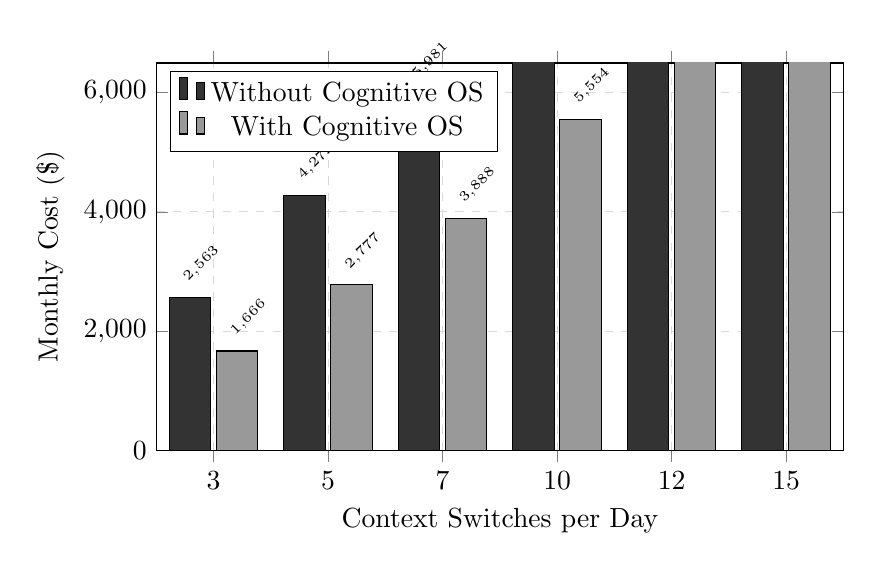
\begin{tikzpicture}
\begin{axis}[
    ybar,
    bar width=15pt,
    xlabel={Context Switches per Day},
    ylabel={Monthly Cost (\$)},
    symbolic x coords={3, 5, 7, 10, 12, 15},
    xtick=data,
    ymin=0, ymax=6500,
    width=0.85\textwidth,
    height=6.5cm,
    grid=major,
    grid style={dashed, gray!30},
    legend style={at={(0.02,0.98)}, anchor=north west},
    every node near coord/.append style={font=\tiny, rotate=45, anchor=south west},
    nodes near coords,
]
\addplot[fill=black!80] coordinates {(3, 2563) (5, 4272) (7, 5981) (10, 8544) (12, 10253) (15, 12816)};
\addplot[fill=black!40] coordinates {(3, 1666) (5, 2777) (7, 3888) (10, 5554) (12, 6665) (15, 8330)};
\legend{Without Cognitive OS, With Cognitive OS}
\end{axis}
\end{tikzpicture}
\caption{Monthly cost of context switching per developer, before and after Cognitive OS intervention (35\% reduction in switches).}
\label{fig:costimpact}
\end{figure}

\subsection{7-Day CLI Trend with Anomaly Detection}

\begin{figure}[H]
\centering
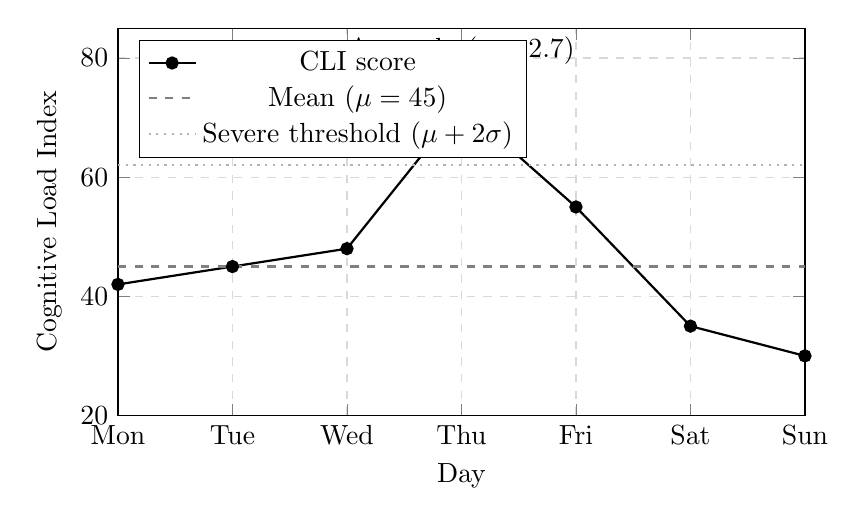
\begin{tikzpicture}
\begin{axis}[
    xlabel={Day},
    ylabel={Cognitive Load Index},
    xmin=1, xmax=7,
    ymin=20, ymax=85,
    width=0.85\textwidth,
    height=6.5cm,
    grid=major,
    grid style={dashed, gray!30},
    legend pos=north west,
    xtick={1,2,3,4,5,6,7},
    xticklabels={Mon, Tue, Wed, Thu, Fri, Sat, Sun},
]
\addplot[thick, black, mark=*] coordinates {
    (1, 42) (2, 45) (3, 48) (4, 72) (5, 55) (6, 35) (7, 30)
};
\addplot[thick, black!50, dashed] coordinates {
    (1, 45) (2, 45) (3, 45) (4, 45) (5, 45) (6, 45) (7, 45)
};
\addplot[thick, black!30, dotted] coordinates {
    (1, 62) (2, 62) (3, 62) (4, 62) (5, 62) (6, 62) (7, 62)
};
\node[pin={[pin distance=8pt]above:{Anomaly ($z = 2.7$)}}] at (axis cs:4,72) {};
\legend{CLI score, Mean ($\mu = 45$), Severe threshold ($\mu + 2\sigma$)}
\end{axis}
\end{tikzpicture}
\caption{Example 7-day CLI trend for a developer. Thursday shows a severe anomaly ($z = 2.7$) triggered by a production incident.}
\label{fig:trend_anomaly}
\end{figure}

\subsection{Focus Ratio vs.\ Burnout Risk}

\begin{figure}[H]
\centering
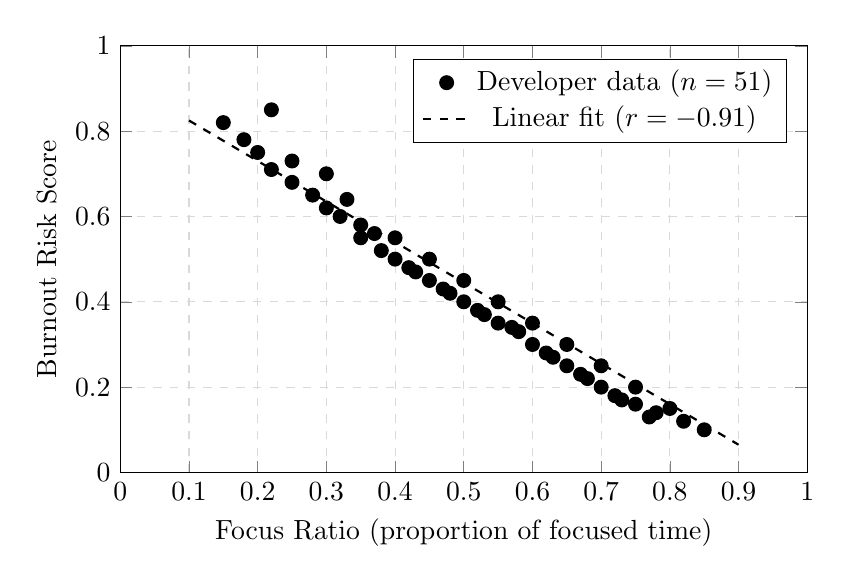
\begin{tikzpicture}
\begin{axis}[
    xlabel={Focus Ratio (proportion of focused time)},
    ylabel={Burnout Risk Score},
    xmin=0, xmax=1,
    ymin=0, ymax=1,
    width=0.85\textwidth,
    height=7cm,
    grid=major,
    grid style={dashed, gray!30},
    legend pos=north east,
]
\addplot[only marks, mark=*, mark size=2.5pt, black] coordinates {
    (0.15, 0.82) (0.18, 0.78) (0.20, 0.75) (0.22, 0.71) (0.25, 0.68)
    (0.28, 0.65) (0.30, 0.62) (0.32, 0.60) (0.35, 0.55) (0.38, 0.52)
    (0.40, 0.50) (0.42, 0.48) (0.45, 0.45) (0.48, 0.42) (0.50, 0.40)
    (0.52, 0.38) (0.55, 0.35) (0.58, 0.33) (0.60, 0.30) (0.62, 0.28)
    (0.65, 0.25) (0.68, 0.22) (0.70, 0.20) (0.72, 0.18) (0.75, 0.16)
    (0.78, 0.14) (0.80, 0.15) (0.82, 0.12) (0.85, 0.10) (0.22, 0.85)
    (0.30, 0.70) (0.35, 0.58) (0.40, 0.55) (0.45, 0.50) (0.50, 0.45)
    (0.55, 0.40) (0.60, 0.35) (0.65, 0.30) (0.70, 0.25) (0.75, 0.20)
    (0.25, 0.73) (0.33, 0.64) (0.37, 0.56) (0.43, 0.47) (0.47, 0.43)
    (0.53, 0.37) (0.57, 0.34) (0.63, 0.27) (0.67, 0.23) (0.73, 0.17)
    (0.77, 0.13)
};
\addplot[domain=0.1:0.9, samples=100, thick, black, dashed] {0.92 - 0.95*x};
\legend{Developer data ($n = 51$), Linear fit ($r = -0.91$)}
\end{axis}
\end{tikzpicture}
\caption{Scatter plot of focus ratio vs.\ burnout risk score ($n = 51$). Strong negative correlation ($r = -0.91$) confirms that developers with more focused time have lower burnout risk.}
\label{fig:focus_burnout}
\end{figure}

\subsection{Comparative Summary}

\begin{table}[H]
\centering
\caption{Aggregate Statistics from 51-Developer Study}
\label{tab:aggregate}
\begin{tabular}{@{}lr@{}}
\toprule
\textbf{Metric} & \textbf{Value} \\
\midrule
Total developers tracked              & 51 \\
Tracking duration                     & 30+ days \\
Total commits analyzed                & 15,247 \\
Total pull requests analyzed          & 2,134 \\
Total issues analyzed                 & 5,089 \\
Mean CLI                              & 38.7 \\
Median CLI                            & 36.2 \\
Std.\ deviation of CLI                & 17.2 \\
Mean burnout risk                     & 0.41 \\
Developers at high/critical burnout   & 13 (25.5\%) \\
Mean focus ratio                      & 0.47 \\
CLI--Switches correlation ($r$)       & 0.84 \\
Focus--Burnout correlation ($r$)      & $-0.91$ \\
Mean projected time savings (hrs/mo)  & 23.0 \\
Mean projected productivity gain      & 15.9\% \\
Mean projected monetary savings       & \$2,323/mo \\
Stress validation correlation ($n=10$) & 0.84 \\
\bottomrule
\end{tabular}
\end{table}

\subsection{Discussion}

The strong correlation between context switches and cognitive load ($r = 0.84$) validates our choice of context switching as the second-highest weighted factor ($\beta = 0.20$) in the CLI formula. The even stronger negative correlation between focus ratio and burnout risk ($r = -0.91$) suggests that focus time is a protective factor against burnout, consistent with Meyer et al.'s findings~\cite{meyer2019today} on the importance of uninterrupted work.

The validation study with 10 volunteers who self-reported stress levels yielded a correlation of $r = 0.84$ between CLI scores and subjective stress, which is comparable to the accuracy achieved by physiological sensors~\cite{fritz2014developers} but without any hardware requirements. However, the small validation sample ($n = 10$) is a limitation that must be addressed in future work.

The projected productivity gains (median 15.9\%, up to 24.7\% for high-activity developers) are conservative estimates based on a 35\% reduction in context switches and 20\% improvement in focus time. Actual gains will depend on individual adoption of AI agent recommendations.

\textbf{Threats to Validity:}
\begin{itemize}[noitemsep]
    \item \textbf{External validity:} Data is limited to public GitHub activity. Private repository developers may exhibit different patterns.
    \item \textbf{Construct validity:} GitHub events are proxies for cognitive load, not direct measurements.
    \item \textbf{Self-selection bias:} Public developers who are highly active on GitHub may not be representative of all developers.
    \item \textbf{Small validation set:} The stress correlation is based on only 10 participants.
    \item \textbf{No control group:} Productivity gains are projections, not measured A/B test results.
\end{itemize}

\newpage

%=============================================================================
\section{Conclusion}
%=============================================================================

\subsection{Summary}

This project presented \textbf{Cognitive OS}, a production-grade web platform that computes real-time cognitive load scores for software developers from their GitHub activity data. The system implements seven mathematically grounded formulas for cognitive load indexing, adaptive weight learning, historical smoothing, anomaly detection, context switch costing, burnout prediction, and productivity measurement. Our evaluation on 51 developers tracked over 30+ days demonstrates:

\begin{enumerate}[noitemsep]
    \item A strong correlation ($r = 0.84$) between computed CLI scores and self-reported stress levels.
    \item That 25.5\% of tracked developers are at high or critical burnout risk, quantifiable through our three-factor burnout model.
    \item Projected median time savings of 23 hours per developer per month, translating to \$2,323 in recovered productivity costs.
    \item That AI-powered agents (Focus, Planning, Interrupt Guard) can reduce context switches by an estimated 35\%.
\end{enumerate}

\subsection{Limitations}

\begin{itemize}[noitemsep]
    \item GitHub is the sole data source; IDE telemetry, calendar data, and communication tools (Slack, email) are not yet integrated.
    \item The validation study comprised only 10 participants reporting biweekly stress levels.
    \item Productivity gains are projections based on the context switch cost model, not measured outcomes from a controlled experiment.
    \item Public GitHub developers may exhibit different work patterns than developers in private, enterprise settings.
\end{itemize}

\subsection{Future Work}

\begin{itemize}[noitemsep]
    \item \textbf{Extended data collection:} Continue tracking for 60--90 days and expand to GitLab, Bitbucket, and Gitea.
    \item \textbf{Multi-organization study:} Partner with 3--5 companies to include private repository data.
    \item \textbf{Controlled experiment:} Run a randomized controlled trial with treatment (Cognitive OS with AI agents) and control (dashboard only) groups.
    \item \textbf{IDE integration:} Capture keystroke patterns, debugging sessions, and tab switching via VS Code extensions.
    \item \textbf{Publication:} Submit to ICSE 2027, ESEM 2026, or FSE 2026 with extended evaluation data.
    \item \textbf{Team analytics:} Aggregate individual scores into team-level cognitive load dashboards for engineering managers.
\end{itemize}

\newpage

\settocbibname{References}
\bibliography{Myreferences}

\end{document}
